\documentclass[journal]{IEEEtran}
\usepackage[utf8]{inputenc}
\usepackage[T1]{fontenc}
\usepackage{textcomp,amsmath,booktabs,array,graphicx,url,microtype,multirow}
\usepackage{tikz}
\usetikzlibrary{positioning,arrows.meta,fit,calc}
\usepackage[hidelinks]{hyperref}

\newcommand{\systemname}{CURIE}

\begin{document}

\title{Missingness-Aware SOFA Reconstruction Across Two ICU Databases
With a Locked Alert-Governance Evaluation in MIMIC-IV}

\author{Satya~Venkata~Ranga~Janaki~Sriram~Mentey
\thanks{S.~V.~R.~J.~S.~Mentey is an independent researcher, Austin, TX 78729, USA
(e-mail: srirammentey@ieee.org; ORCID: 0009-0007-2681-006X).}}

\markboth{IEEE Journal of Biomedical and Health Informatics}
{Mentey: Missingness-Aware SOFA Reconstruction and Alert Governance}

\maketitle

\begin{abstract}
Electronic-health-record implementations of deterministic severity scores
must distinguish an observed normal value from a value that was never
observed, and alert evaluations must distinguish score generation from
clinician interruption. We implemented availability-time Sequential Organ Failure Assessment
reconstruction
with explicit partial and insufficient-data states, versioned rules, evidence
provenance, and a separate alert-governance layer. Component observability was
audited in MIMIC-IV 3.1 and a seeded 8,000-stay eICU-CRD 2.0 sample.
Governance was selected on development and calibration anchor-year groups and
evaluated once on a locked MIMIC-IV test set (14,407 stays; 5,315 labeled
positive). Respiratory and hepatic inputs were the least observable components
in both sources. Governed sensitivity was 98.49\% (95\% confidence interval,
98.15--98.81\%)
versus 98.51\% for threshold-only scoring, and interruptive emissions were
7.67\% of the naive interruptive baseline (95\% confidence interval, 7.54--7.79\%). However,
interruptive sensitivity was 71.36\%, precision was 6.08\%, and 57.4
interruptions were emitted per positive stay reached by an interruption. Post hoc analyses
showed that requiring an alert at least 2 hours before onset reduced governed
sensitivity to 54.43\% and interruptive sensitivity to 10.89\%. Against
discharge sepsis codes, 97.69\% of code-positive stays had a governed alert,
but so did 80.46\% of code-negative stays. These results characterize a
retrospective research prototype, not clinical validity or utility. Explicit
missingness, separate routing endpoints, and lead-time-gated reporting prevent
a high loose-window detection rate from concealing data, timing, and
interruption-burden limitations.
\end{abstract}

\begin{IEEEkeywords}
alert fatigue, clinical decision support, data completeness, eICU-CRD,
electronic health records, MIMIC-IV, reproducibility, SOFA
\end{IEEEkeywords}

\section{Introduction}

\IEEEPARstart{T}{he} Sequential Organ Failure Assessment (SOFA) score combines
respiratory, coagulation, hepatic, cardiovascular, neurologic, and renal
measurements into a deterministic representation of organ
dysfunction~\cite{vincent1996sofa}. The scoring table is simple;
reconstructing it from longitudinal electronic health record (EHR) data is
not. Measurements arrive at different frequencies, documentation time may
differ from physiological event time, drug doses use heterogeneous units, and
the absence of a measurement can be mistaken for a normal result. EHR
completeness is therefore a property of the measurement process and intended
use, not merely the fraction of populated database
fields~\cite{weiskopf2013,kahn2016}.

A second ambiguity appears after scoring. A threshold crossing, a retained
alert record, and an interruptive notification are different events. Treating
them as interchangeable hides the mechanisms that create alert fatigue and
prevents a meaningful accounting of clinician
interruptions~\cite{embi2012,elias2019,ancker2017}. Evaluations of deployed
sepsis decision support likewise show that detection performance alone does
not establish workflow benefit~\cite{downing2019,wong2021}.

This paper evaluates a biomedical-informatics boundary rather than a new
clinical score. The \systemname{} prototype reconstructs SOFA using only
information available at each event time, reports missing components instead
of silently assigning reassuring values, and applies a separately versioned
governance policy to passive and interruptive outputs. The evaluation uses
MIMIC-IV 3.1~\cite{mimiciv31,johnson2023mimiciv} and eICU-CRD
2.0~\cite{eicu20,pollard2018eicu}. Its contributions are:

\begin{enumerate}
\item an explicit data-state contract for deterministic EHR scoring, including
availability time, evidence lineage, and abstention when required inputs are
unobserved;
\item a cross-source audit showing which SOFA inputs the adapters can actually
recover, with eICU-CRD used only to assess extraction portability;
\item a locked MIMIC-IV evaluation that separates threshold crossings,
governed records, and interruptive emissions, with prespecified ablations;
\item post hoc timing and label-sensitivity analyses that quantify how much of
the loose-window detection rate reflects actionable lead time and how
specific stay-level alerting is against an independently coded label; and
\item a reproducibility contract linking the protocol, data/index version,
label implementation, rule version, operating point, bootstrap seed, and
every reported aggregate.
\end{enumerate}

No language model generates, suppresses, or modifies an alert. We do not
claim diagnostic accuracy, clinical validation, improved outcomes,
production readiness, or regulatory readiness.

\section{Related Work}

\subsection{SOFA reconstruction and missing data}
SOFA was designed for daily bedside charting~\cite{vincent1996sofa}, and serial
SOFA carries prognostic information~\cite{ferreira2001}. Retrospective
studies commonly compute it from EHR extracts using shared concept code; the
MIMIC Code Repository provides such SQL for MIMIC and was introduced to make
derived concepts reproducible~\cite{johnson2018code}. A recurring convention
treats an unmeasured component as normal (a subscore of zero), which Lambden
\emph{et al.} identify as a source of bias in clinical trials and
observational research~\cite{lambden2019}. Data-quality frameworks separate
conformance, completeness, and plausibility~\cite{kahn2016} and define
completeness relative to a task~\cite{weiskopf2013}. Our scorer does not
propose a new imputation method; it refuses to impute and propagates
component-level missingness into every emitted signal so that downstream
evaluation can condition on it.

\subsection{Sepsis labels and construct overlap}
Sepsis-3 operationalizes sepsis as suspected infection with an acute SOFA
increase of at least two points~\cite{singer2016,seymour2016}. When the
reference label is itself SOFA-derived, a SOFA-based detector shares part of
its construct with the label, so high sensitivity partly reflects
incorporation. Administrative definitions based on discharge codes, such as
explicit sepsis codes or infection-plus-organ-dysfunction
algorithms~\cite{angus2001,martin2003}, have different error profiles and
diverge from clinical surveillance definitions~\cite{rhee2017}; in MIMIC,
sepsis identification methods yield markedly different cohorts and
outcomes~\cite{johnson2018sepsis}. We therefore use discharge codes only as a
label-sensitivity analysis, never as an onset time or as validation.

\subsection{Alert burden and governance mechanisms}
Clinicians override most interruptive alerts~\cite{vandersijs2006}, and
repeated alerts increase fatigue~\cite{ancker2017,embi2012}. Human-factors
guidance recommends reducing redundant and low-value
interruptions~\cite{phansalkar2010}, and health-system studies measure
interruption burden directly~\cite{elias2019}. Refractory periods,
deduplication, and tiered delivery are established design patterns; we do not
claim that any single mechanism is new. Our contribution is to version these
mechanisms as a policy object separate from the score and to attribute burden
to each mechanism by prespecified ablation on a locked test set.

\subsection{Evaluation of sepsis decision support}
Machine-learning early-warning systems have reported strong retrospective
discrimination~\cite{henry2015,nemati2018,moor2021}, and a public benchmark
standardized evaluation on hourly ICU data~\cite{reyna2020}. External
evaluation of a widely deployed proprietary model found substantially lower
performance and a large alert burden~\cite{wong2021}, whereas a prospective
multi-site study associated a deployed system with outcomes when alerts were
acted upon~\cite{adams2022}. Reporting guidance emphasizes intended use,
data provenance, and transparent evaluation~\cite{collins2024,wiens2019}. The
present study is positioned before such evaluations: it characterizes data
availability, timing, and interruption burden of a deterministic pipeline so
that a later prospective study can be designed around measurable quantities.

\section{System and Methods}

\subsection{System boundary and information flow}

Fig.~\ref{fig:system} and Table~\ref{tab:boundary} define the evaluated
stages. The separation is intentional: a scorer answers what can be computed
from the observed record; governance answers how a completed signal is
routed. An optional language-model component in the larger prototype was
disabled and is outside the alert path.

\begin{figure*}[t]
\centering
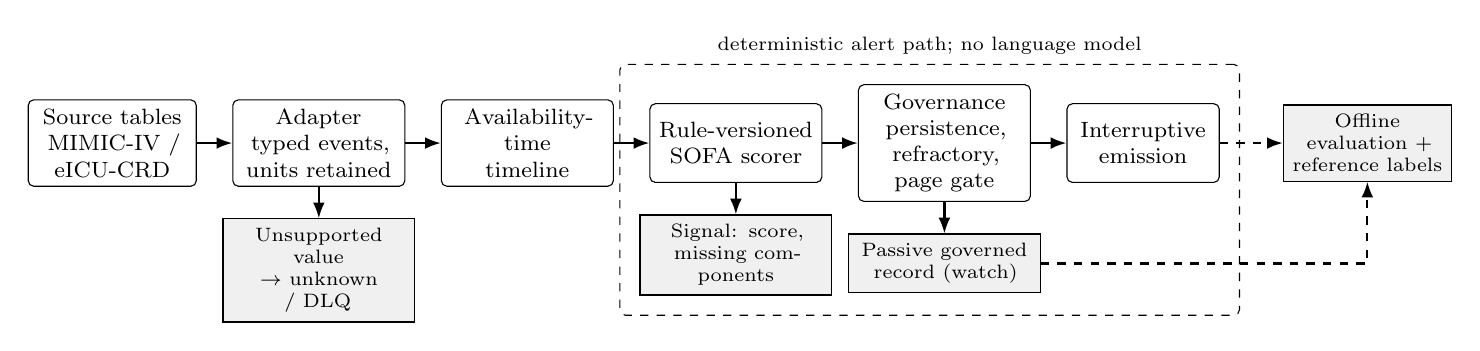
\begin{tikzpicture}[
  node distance=5mm and 4.5mm,
  box/.style={draw, rounded corners=2pt, align=center, font=\footnotesize,
              minimum height=10mm, text width=19.5mm, fill=white},
  store/.style={draw, align=center, font=\scriptsize, text width=22mm,
                minimum height=7mm, fill=gray!12},
  arr/.style={-{Latex[length=2mm]}, thick},
  lab/.style={font=\scriptsize, align=center}
]
\node[box, text width=19mm] (src) {Source tables\\MIMIC-IV /\\eICU-CRD};
\node[box, right=of src] (adp) {Adapter\\typed events,\\units retained};
\node[box, right=of adp] (tl) {Availability-time\\timeline};
\node[box, right=of tl] (sc) {Rule-versioned\\SOFA scorer};
\node[box, right=of sc] (gov) {Governance\\persistence,\\refractory, page gate};
\node[box, right=of gov, text width=17mm] (page) {Interruptive\\emission};
\node[store, below=4mm of gov] (watch) {Passive governed\\record (watch)};
\node[store, below=4mm of sc] (sig) {Signal: score,\\missing components};
\node[store, below=4mm of adp] (dlq) {Unsupported value\\$\rightarrow$ unknown / DLQ};
\node[store, right=8mm of page, text width=19mm] (eval) {Offline\\evaluation +\\reference labels};
\draw[arr] (src) -- (adp);
\draw[arr] (adp) -- (tl);
\draw[arr] (tl) -- (sc);
\draw[arr] (sc) -- (gov);
\draw[arr] (gov) -- (page);
\draw[arr] (gov) -- (watch);
\draw[arr] (sc) -- (sig);
\draw[arr] (adp) -- (dlq);
\draw[arr, dashed] (page) -- (eval);
\draw[arr, dashed] (watch.east) -| (eval.south);
\node[draw, dashed, rounded corners=2pt, fit=(sc)(gov)(page)(sig)(watch),
      inner sep=2.5mm, label={[font=\scriptsize]above:deterministic alert path; no language model}] {};
\end{tikzpicture}
\caption{Information flow. Each emitted signal carries its score, component
values, missing-component list, rule version, and source-observation
identifiers. Governance may delay, deduplicate, or demote a signal to a
passive record but cannot change its score or evidence. Reference labels are
joined to the outputs only offline, for evaluation (dashed arrows), and are
never visible to the timeline or scorer.}
\label{fig:system}
\end{figure*}

\begin{table}[t]
\centering
\caption{Deterministic processing boundary.}
\label{tab:boundary}
\footnotesize
\begin{tabular}{@{}p{0.16\columnwidth}p{0.27\columnwidth}p{0.45\columnwidth}@{}}
\toprule
Stage & Input/output & Invariant \\
\midrule
Adapter & Source rows $\rightarrow$ typed events & Units and source times are retained; unsupported values remain unknown. \\
Timeline & Typed events $\rightarrow$ state & Only observations available by the scoring time are visible. \\
Scorer & State $\rightarrow$ SOFA signal & Missing inputs yield component-level missingness and partial status, not an assumed score of zero. \\
Governance & Signal $\rightarrow$ watch/page decision & Routing may delay or deduplicate a complete signal but cannot change its score or evidence. \\
Episode layer & Decisions $\rightarrow$ episodes & Repeated signals are grouped without erasing the underlying records. \\
\bottomrule
\end{tabular}
\end{table}

Poison or unsupported input is rejected to a dead-letter queue rather than
converted to a normal clinical value. Python reference scorers and Java/Flink
streaming implementations are checked against shared golden fixtures, and a
rule bundle cannot be activated unless this parity gate passes.

\subsection{Datasets, cohort, and split policy}

MIMIC-IV 3.1 contains deidentified data from a single US academic medical
center; eICU-CRD 2.0 contains deidentified data from more than 200 US
hospitals. Both require credentialed PhysioNet access and a signed data-use
agreement. The frozen protocol included adults, required valid ICU admission
and discharge times and an ICU duration of at least four hours, and retained
the earliest eligible ICU stay per hospital admission. MIMIC's
deidentification shifts calendar dates independently per patient;
development, calibration, and test assignment therefore used each patient's
\texttt{anchor\_year\_group} (2008--2010 and 2011--2013, 2014--2016, and
2017--2019, respectively) rather than shifted calendar years. Because the
group is a patient attribute, the splits are patient-disjoint; because it
locates only the patient's anchor year, the temporal ordering of individual
stays is approximate. Table~\ref{tab:flow} gives
every denominator.

\begin{table}[t]
\centering
\caption{MIMIC-IV cohort flow (protocol v2 selection).}
\label{tab:flow}
\footnotesize
\begin{tabular}{@{}lr@{}}
\toprule
Step & ICU stays \\
\midrule
ICU stays in source & 94,458 \\
\quad Excluded: invalid admission/discharge time & 14 \\
\quad Excluded: ICU duration $<$ 4 h & 714 \\
\quad Excluded: later eligible stay, same admission & 8,689 \\
Protocol cohort & 85,041 \\
\quad Not assigned: anchor-year group 2020--2022 & 9,566 \\
Study cohort & 75,475 \\
\quad Development (2008--2013) & 44,755 \\
\quad Calibration (2014--2016) & 16,313 \\
\quad Locked test (2017--2019) & 14,407 \\
\bottomrule
\end{tabular}
\end{table}

An earlier cohort audit selected the first ICU stay per admission before the
time filters and retained 84,855 stays. All 84,855 are in the protocol cohort;
the protocol rule adds 186 admissions whose first ICU stay was invalid or
shorter than four hours but whose later stay was eligible. The cohort-wide
completeness audit below uses the earlier 84,855-stay selection. eICU-CRD was
sampled with a fixed seed (8,000 stays, seed 42) for an extraction-completeness
analysis only.

\subsection{Availability-time SOFA reconstruction}

At each incoming event time, the timeline selects the most recent usable
value within the component's documented lookback rule. A value is usable only
after the time at which it would have been available to the scoring system;
laboratory and charted values defer to their storage time, which prevents a
later result or correction from entering an earlier score. When no usable
value exists, the component is marked missing, and the total is emitted with
its completeness state; it is never represented as a fully observed score.

Respiration prioritizes PaO$_2$/FiO$_2$. A SpO$_2$/FiO$_2$ fallback uses the
published relationship only within its supported saturation
range~\cite{rice2007}; FiO$_2$ is never inferred from missing oxygen
documentation. Cardiovascular processing preserves the source vasopressor
unit and converts only combinations covered by an explicit unit policy.
Vasopressin rates that cannot be converted without an unavailable
concentration remain unknown. Urine-output windows require coverage for the
specified duration. These choices make missingness visible but do not
establish that a reconstructed component is clinically correct.

\subsection{Completeness and portability audit}

For each SOFA input we measured, cohort-wide in MIMIC-IV, the fraction of
stays with at least one usable observation and the fraction observed during
the first ICU day. In seeded 8,000-stay samples from each database we replayed
the scorer and recorded, per component, the fraction of stays whose final
score of the stay lacked a usable value within that component's lookback
window. We also reconciled indexed-loader output against a
direct source-table scan for a deterministic 25-stay sample. The eICU audit
exercised the same typed-event and scoring contracts through source-specific
extraction mappings. It did not evaluate labels, governance, outcomes, or
cross-site clinical performance.

\subsection{Governance policy and locked evaluation}

The governance layer maintains trajectory persistence, refractory state, and
episode membership. A governed record is a retained, non-duplicative alert
event. An interruptive emission additionally satisfies the page gate, which
can require repeated crossings, sustained elevation, and a rising
trajectory. The selected policy used a 90-min refractory interval and a page
gate requiring two crossings sustained for 30 min with a rising score.
Removing or delaying an interruption does not alter the underlying signal.

The protocol, candidate policies, and ablations were specified and frozen
before locked test evaluation. Candidates were developed on development
groups, one operating point was selected on calibration (minimum interruptive
ratio subject to the sensitivity criterion), and the test split was evaluated
once. The primary detection window was 12 h before through 6 h after the
Sepsis-3-aligned onset generated from a pinned MIMIC Code Repository
revision~\cite{johnson2018code,seymour2016}. The primary endpoints were
governed sensitivity (success if within 10 percentage points of threshold-only
sensitivity or at least 70\%) and the ratio of interruptive emissions under
governance to the naive interruptive baseline (success if at most 25\%). This
endpoint is not the ratio of all governed records to all raw threshold
crossings; both are reported.

Sensitivity is the fraction of labeled-positive stays with at least one
qualifying event in the window. Burden is reported as counts and rates per 100
patient-days. Interruptive precision is the fraction of interruptive
emissions that fall inside a labeled-positive stay's detection window. Number
needed to alert (NNA) is interruptive emissions divided by labeled-positive
stays with at least one in-window interruptive emission (3,793 under full
governance); it is a burden statistic, not a treatment effect.

\subsection{Post hoc secondary analyses}

After the locked evaluation, and without changing the operating point, we
replayed the test split once more with the frozen policy and defined three
secondary analyses. None was used for selection.

\emph{Lead-time gate.} A labeled-positive stay counts as detected only if an
alert occurs in $[t_{\mathrm{onset}}-12\,\mathrm{h},\,
t_{\mathrm{onset}}-2\,\mathrm{h}]$. This removes credit for alerts coincident
with, or after, the label.

\emph{Discharge-code label sensitivity.} A stay is code-positive if its
hospital admission carries at least one code from a frozen ICD-9/10 list of
explicit sepsis, severe-sepsis, and septic-shock codes (ICD-9 038.x, 995.91,
995.92, 785.52; ICD-10 A40--A41, R65.20, R65.21, O85). Because discharge
codes have no onset time, we report the fraction of code-positive stays with
any alert during the ICU stay, alongside the same fraction in code-negative
stays. Codes were never features and were joined only after replay.

\emph{Subgroups.} Detection and burden were summarized by sex and age band.
These summaries are descriptive and not powered for between-group inference.

\subsection{Statistics and reproducibility}

Confidence intervals are stay-level percentile bootstrap intervals (1,000
replicates, seed 42). Every number in this paper resolves to one of two
content-hashed sidecars: the locked study manifest (primary endpoints,
ablations, bootstrap intervals, miss count) and a publication-aggregate
sidecar (cohort flow, characteristics, completeness, post hoc analyses, and
subgroups). The latter records the SHA-256 of each audit input, the index
hash, the label-artifact hash, and the operating-point hash, and reproduces
the frozen governed sensitivity from the replay rows before it can be
written. Cells describing fewer than 11 stays are suppressed.

\section{Results}

\subsection{Cohort}

Table~\ref{tab:chars} describes the three splits. Median age and sex
distribution were similar across splits, whereas Sepsis-3 label prevalence
was lower in the locked test groups (36.9\%) than in development (48.0\%)
and calibration (45.5\%). The test split contained 14,407 stays, 5,315
labeled-positive stays, and 54,401 patient-days.

\begin{table}[t]
\centering
\caption{Cohort characteristics by split. Values are n, n (\%), or median
[interquartile range].}
\label{tab:chars}
\footnotesize
\setlength{\tabcolsep}{3pt}
\begin{tabular}{@{}lrrr@{}}
\toprule
 & Development & Calibration & Test \\
\midrule
ICU stays & 44,755 & 16,313 & 14,407 \\
Patients & 31,223 & 13,157 & 12,165 \\
Age, y & 64 [52--75] & 65 [53--76] & 66 [54--76] \\
Female & 20,305 (45.4) & 7,123 (43.7) & 6,228 (43.2) \\
ICU stay, d & 1.85 [1.05--3.43] & 1.92 [1.11--3.69] & 2.03 [1.14--4.01] \\
Sepsis-3 positive & 21,484 (48.0) & 7,426 (45.5) & 5,315 (36.9) \\
\bottomrule
\end{tabular}
\end{table}

\subsection{Component observability}

Table~\ref{tab:completeness} reports input observability and scored
component missingness. Cardiovascular, neurologic, coagulation, and renal
components were missing in fewer than 5\% of scored stays in both databases.
The respiratory component was missing in 66.4\% of scored MIMIC-IV stays and
59.7\% of scored eICU-CRD stays, driven by sparse FiO$_2$ documentation, and
the hepatic component in 13.4\% and 27.6\%, respectively. The final score
of the stay was fully observed in 30.2\% (MIMIC-IV) and 29.8\% (eICU-CRD)
of sampled stays. Observability describes the available record; it
does not show that observed components were accurate.

\begin{table}[t]
\centering
\caption{Input observability (\%, MIMIC-IV cohort-wide, 84,855 stays) and
component missingness in the final score of each stay (\%, seeded
8,000-stay samples).}
\label{tab:completeness}
\footnotesize
\setlength{\tabcolsep}{3pt}
\begin{tabular}{@{}llrrrr@{}}
\toprule
 & & \multicolumn{2}{c}{MIMIC input observed} & \multicolumn{2}{c}{Component missing} \\
\cmidrule(lr){3-4}\cmidrule(l){5-6}
Component & Input & Any & Day 1 & MIMIC & eICU \\
\midrule
Respiration & PaO$_2$ & 70.6 & 53.8 & \multirow{2}{*}{66.4} & \multirow{2}{*}{59.7} \\
 & FiO$_2$ & 49.3 & 45.7 & & \\
Coagulation & Platelets & 99.7 & 96.5 & 0.1 & 4.1 \\
Liver & Bilirubin & 80.9 & 44.0 & 13.4 & 27.6 \\
Cardiovascular & MAP & 99.8 & 99.5 & 0.2 & 1.7 \\
CNS & GCS & 99.8 & 99.7 & 0.2 & 0.9 \\
Renal & Creatinine & 99.8 & 97.2 & \multirow{2}{*}{$<$0.1} & \multirow{2}{*}{1.8} \\
 & Urine output & 96.5 & 95.5 & & \\
\midrule
\multicolumn{4}{@{}l}{Fully observed final score} & 30.2 & 29.8 \\
\bottomrule
\end{tabular}
\end{table}

In the MIMIC-IV vasopressor audit, 685,045 infusion rows mapped to a
supported dose representation and 31,020 remained explicitly unknown, of which
30,559 were vasopressin rates recorded in units per hour without a usable
concentration. The source-to-index reconciliation sample had no missing or
extra rows. These engineering checks reduce silent transformation error; they
are not a comparison with bedside adjudication.

\subsection{Locked MIMIC-IV governance evaluation}

Table~\ref{tab:primary} separates the output levels. Both primary endpoints
were met. The all-record reduction was 784,548 governed records divided by
4,351,252 threshold crossings, or 18.03\%. The prespecified interruptive
endpoint was 217,778 divided by 2,840,825 naive interruptive emissions, or
7.67\% (95\% CI, 7.54--7.79\%).

\begin{table}[t]
\centering
\caption{Locked MIMIC-IV test results (14,407 stays). CI denotes the
prespecified stay-level bootstrap interval; intervals were prespecified only
for the rows that show one.}
\label{tab:primary}
\footnotesize
\begin{tabular}{p{0.52\columnwidth}r}
\toprule
Metric & Result \\
\midrule
Threshold-only sensitivity & 98.51\% \\
Governed sensitivity (95\% CI) & 98.49\% (98.15--98.81) \\
Interruptive sensitivity & 71.36\% \\
Raw threshold crossings & 4,351,252 \\
Governed records & 784,548 \\
Governed/raw record ratio & 18.03\% \\
Naive interruptive emissions & 2,840,825 \\
Governed interruptive emissions & 217,778 \\
Interruptive ratio (95\% CI) & 7.67\% (7.54--7.79) \\
Governed records per 100 patient-days & 1,442.2 \\
Interruptions per 100 patient-days & 400.3 \\
Interruptive precision & 6.08\% \\
Interruptive NNA (95\% CI) & 57.4 (55.6--59.4) \\
\bottomrule
\end{tabular}
\end{table}

Governance retained 5,235 of 5,315 labeled-positive stays within the loose
window, leaving 80 without a governed detection (1.51\%). The near-equivalence
of governed and threshold-only sensitivity applies to passive governed
records. It does not apply to clinician interruption: the page gate reduced
interruptive sensitivity to 71.36\% while still producing 400.3 interruptions
per 100 patient-days.

\subsection{Prespecified ablations}

Table~\ref{tab:ablation} attributes burden to mechanisms. The refractory
interval was the only deduplicating mechanism: removing it returned governed
records to the raw crossing count and raised interruptive emissions from
217,778 to 1,555,348. Removing the page gate more than doubled interruptive
emissions (469,718) and raised interruptive sensitivity to 78.53\% at lower
precision (4.45\%). Six ablations produced results identical to full
governance because the mechanism was already inactive in the selected policy
(trajectory persistence, multiple crossings, baseline delta) or did not alter
any emission in this replay (context suppression, episode arbitration,
late-event buffer).

\begin{table}[t]
\centering
\caption{Prespecified ablations on the locked test split. Sens., sensitivity
(\%); Int., interruptive; ratio, interruptive emissions relative to the naive
interruptive baseline (\%).}
\label{tab:ablation}
\footnotesize
\setlength{\tabcolsep}{2.5pt}
\begin{tabular}{@{}lrrrrrr@{}}
\toprule
Policy & Gov. sens. & Int. sens. & Records & Int. & Ratio & NNA \\
\midrule
Threshold-only & 98.51 & 80.30 & 4,351,252 & 2,840,825 & 100.0 & 665.6 \\
Full governance & 98.49 & 71.36 & 784,548 & 217,778 & 7.67 & 57.4 \\
$-$Refractory & 98.51 & 74.98 & 4,351,252 & 1,555,348 & 54.75 & 390.3 \\
$-$Page gate & 98.49 & 78.53 & 784,548 & 469,718 & 16.53 & 112.5 \\
Six others\,$^{a}$ & 98.49 & 71.36 & 784,548 & 217,778 & 7.67 & 57.4 \\
\bottomrule
\multicolumn{7}{@{}p{0.95\columnwidth}@{}}{\scriptsize $^{a}$Persistence,
crossings, baseline, context suppression, episode arbitration, late-event
buffer.}
\end{tabular}
\end{table}

\subsection{Lead time and label sensitivity (post hoc)}

Fig.~\ref{fig:lead} shows the lead of the earliest governed alert in the
detection window. The median lead among the 5,235 detected stays was 2.68 h
(interquartile range, 0.85--7.23 h), and in 120 stays the earliest in-window
alert followed onset. Requiring at least 2 h of lead reduced governed
sensitivity from 98.49\% to 54.43\% and interruptive sensitivity from
71.36\% to 10.89\% (Table~\ref{tab:sensitivity}). Thus, nearly half of the
loose-window detections occurred within 2 h of, or after, the label.

\begin{figure}[t]
\centering
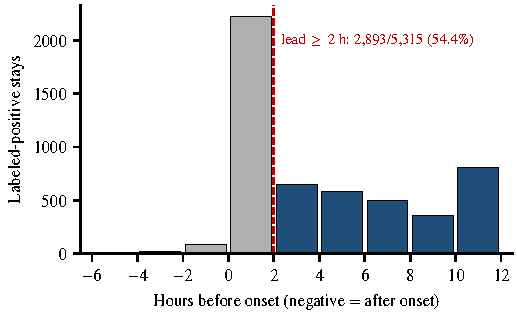
\includegraphics[width=\columnwidth]{figures/lead_time_distribution.pdf}
\caption{Lead of the earliest governed alert relative to Sepsis-3-aligned
onset among 5,235 detected test stays. Grey bars fall short of the 2-h lead
gate. The rightmost bin is right-censored by the 12-h detection window.}
\label{fig:lead}
\end{figure}

\begin{table}[t]
\centering
\caption{Post hoc timing and label-sensitivity analyses on the locked test
split. Values are \% (95\% stay-bootstrap CI) where shown; rows without an
interval are descriptive point estimates that were not bootstrapped.}
\label{tab:sensitivity}
\footnotesize
\setlength{\tabcolsep}{3pt}
\begin{tabular}{@{}p{0.58\columnwidth}r@{}}
\toprule
Analysis & Result \\
\midrule
\multicolumn{2}{@{}l}{\emph{Sepsis-3 onset (5,315 positive stays)}} \\
Governed, primary window & 98.49 (98.15--98.81) \\
Governed, lead $\geq$ 2 h & 54.43 (53.02--55.79) \\
Interruptive, primary window & 71.36 \\
Interruptive, lead $\geq$ 2 h & 10.89 (10.08--11.76) \\
\midrule
\multicolumn{2}{@{}l}{\emph{Discharge sepsis codes (2,249 positive stays)}} \\
Any governed alert, code-positive & 97.69 (97.05--98.26) \\
Any governed alert, code-negative (12,158) & 80.46 \\
Any interruptive alert, code-positive & 82.13 (80.46--83.60) \\
Any interruptive alert, code-negative & 51.77 \\
Code- and Sepsis-3-positive (1,843): primary window & 99.62 \\
Code- and Sepsis-3-positive: lead $\geq$ 2 h & 58.82 \\
\midrule
\multicolumn{2}{@{}l}{\emph{Sepsis-3-negative stays (9,092)}} \\
Any governed alert & 73.58 \\
Any interruptive alert & 40.54 \\
\bottomrule
\end{tabular}
\end{table}

Discharge codes and Sepsis-3 labels overlapped only partially: 1,843 stays
were positive by both, 406 by codes only, and 3,472 by Sepsis-3 only. Nearly
all code-positive stays received a governed alert, but so did 80.46\% of
code-negative stays. Interruptive alerts separated the groups more (82.13\%
versus 51.77\%) yet still reached half of code-negative stays. Stay-level
alerting is therefore sensitive but weakly specific against an
independently assigned label.

\subsection{Subgroups}

Table~\ref{tab:subgroups} summarizes detection and burden by sex and age.
Loose-window governed sensitivity was at least 97.8\% in every subgroup.
Lead-gated sensitivity was lower in women than in men (51.67\% versus
56.39\%) and in patients aged 65 years or older than in younger patients.
Interruptive sensitivity was lowest in patients aged 80 years or older
(64.41\%). These differences are descriptive; they may reflect differences in
measurement frequency or label timing and warrant targeted analysis before
any deployment.

\begin{table}[t]
\centering
\caption{Descriptive subgroup results on the locked test split. Sens.,
sensitivity (\%); lead, governed sensitivity with lead $\geq$ 2 h (\%);
Int./100 pd, interruptions per 100 patient-days.}
\label{tab:subgroups}
\footnotesize
\setlength{\tabcolsep}{2.5pt}
\begin{tabular}{@{}lrrrrrr@{}}
\toprule
Group & Stays & Pos. & Gov. sens. & Lead & Int. sens. & Int./100 pd \\
\midrule
Female & 6,228 & 2,210 & 97.87 & 51.67 & 67.29 & 372.5 \\
Male & 8,179 & 3,105 & 98.94 & 56.39 & 74.27 & 420.4 \\
18--44 y & 2,038 & 641 & 97.97 & 60.22 & 71.61 & 346.0 \\
45--64 y & 4,772 & 1,718 & 98.72 & 58.15 & 74.80 & 392.0 \\
65--79 y & 5,113 & 1,877 & 98.77 & 50.83 & 72.14 & 423.6 \\
$\geq$80 y & 2,484 & 1,079 & 97.96 & 51.34 & 64.41 & 413.6 \\
\bottomrule
\end{tabular}
\end{table}

\section{Discussion}

This study supports four technical conclusions. First, a deterministic score
does not eliminate data-quality uncertainty. Explicit component states make
the uncertainty inspectable: fewer than one third of sampled stays ended with
a fully observed SOFA score in either database, almost entirely because of
respiratory and hepatic inputs. A pipeline that silently scored those
components as normal would report complete scores for every stay and bias
severity downward exactly where documentation is sparse~\cite{lambden2019}.

Second, score generation and clinician interruption require separate
endpoints. Governance preserved loose-window detection while emitting 7.67\%
as many interruptions, and the ablations localize this effect to two
mechanisms: refractory deduplication and the page gate. Yet interruptive
precision remained 6.08\% and 400.3 interruptions were emitted per 100
patient-days. Reporting only the sensitivity or only the reduction ratio would
obscure one of these facts.

Third, loose detection windows overstate actionable warning. The primary
window credits alerts up to 6 h after onset. When at least 2 h of lead was
required, governed sensitivity fell to 54.43\% and interruptive sensitivity to
10.89\%. Part of this gap is expected from construct overlap: the
Sepsis-3-aligned onset is defined by the same SOFA rise that triggers the
score, so many alerts coincide with the label by construction. The
discharge-code analysis addresses a different question and gives a
complementary warning: alerts reached nearly every code-positive stay but
also most code-negative stays. Neither analysis validates the detector; both
bound what the primary sensitivity can be taken to mean. We recommend that
governance evaluations report lead-gated and label-negative results next to
any loose-window sensitivity.

Fourth, reproducibility for a rule-based informatics pipeline is more than
publishing source code. The results depend on source version, extraction
semantics, availability time, label implementation, cohort rule, split, rule
bundle, operating point, and metric denominator. A one-rule difference in
stay selection changed the cohort by 186 stays; recording both rules and
reconciling them exactly is what makes that difference auditable. The
evidence package therefore freezes these objects with content hashes, and
corrections are issued as new versions rather than edits.

\subsection{Relation to the companion manuscript}

A separate manuscript, ``Governing Interruptions After Deterministic
Deterioration Scoring: A Retrospective Evaluation on PhysioNet Challenge
2019,'' is under review at the \emph{International Journal of Medical
Informatics} (manuscript IJMEDI-S-26-06829). It evaluates governance of a
partial SOFA score on the hourly PhysioNet Challenge 2019
benchmark~\cite{reyna2020}. The present work does not reuse that cohort, its
holdout results, tables, or figures. Its primary contributions are the EHR
reconstruction and provenance boundary, the cross-database completeness
audit, and a locked MIMIC-IV evaluation with timing and label-sensitivity
analyses.

\section{Limitations}

The study is retrospective and offline. The primary onset label is
SOFA-derived, creating construct overlap with the score under evaluation; the
reported sensitivity is therefore a pipeline-behavior measure, not diagnostic
accuracy. The lead-time, discharge-code, and subgroup analyses were defined
after the locked evaluation and should be read as post hoc. Discharge codes
reflect billing and documentation practice, carry no onset time, and are
themselves an imperfect reference~\cite{rhee2017,johnson2018sepsis}. No
clinician adjudication, prospective shadow deployment, human-factors
assessment, treatment endpoint, mortality endpoint, or comparison with a
deployed commercial system was performed. eICU-CRD was not used for labeled
outcome or governance evaluation, so this paper offers no external validation
of detection or alerting behavior. The cohort-wide completeness audit used an
earlier stay-selection rule that differs from the study cohort by 186 of
85,041 stays. Component observability does not establish measurement
validity, and differing documentation practices limit direct cross-database
comparison. MIMIC-IV reflects a single center, and label prevalence differed
across anchor-year groups.

\section{Conclusion}

An EHR scoring pipeline should expose what it did not observe, and an
alerting evaluation should distinguish what it computed, retained, and sent
interruptively, and when. In a locked MIMIC-IV evaluation, the \systemname{}
research prototype preserved loose-window governed detection while reducing
the prespecified interruptive burden ratio to 7.67\%, but interruptive
precision, absolute notification burden, and lead-gated sensitivity remained
limiting. A two-database completeness audit localized missing-input risk
without treating availability as clinical validity. These findings motivate
prospective workflow and clinical evaluation; they do not provide it.

\section*{Author Contributions}
S.~V.~R.~J.~S.~Mentey: conceptualization, methodology, software, formal
analysis, investigation, data curation, visualization, and writing.

\section*{Data and Code Availability}
MIMIC-IV 3.1 and eICU-CRD 2.0 are available to credentialed users through
PhysioNet under their data-use agreements; patient-level data and replay
outputs are not redistributed. Source code, rule bundles, parity fixtures,
tests, the frozen protocol, operating point, study manifest, and
publication-aggregate sidecar with content hashes, and reproduction commands
are available at
\url{https://github.com/sreeram843/curie-prediction-pipeline}.

\section*{Ethics Statement}
This study is a secondary analysis of deidentified data obtained from
PhysioNet under credentialed-access data-use agreements, with no new data
collection and no contact with participants. Because the analysis
uses only deidentified data and involves no interaction with participants,
it did not require independent ethics review. No new consent was sought; the
source databases were created under approvals that waived individual
consent: MIMIC-IV was approved by the institutional review boards of Beth
Israel Deaconess Medical Center and the Massachusetts Institute of Technology
with a waiver of consent, and eICU-CRD was exempt from institutional review
because of its retrospective design and certified deidentification.

\section*{Funding}
This research received no external funding and was conducted on a self-funded
basis.

\section*{Competing Interests}
The author declares no competing interests.

\section*{Acknowledgment}
Generative AI tools were used in this work under the author's direction:
OpenAI Codex, the Cursor coding agent (using large language models from
multiple vendors), and Anthropic Claude Code. They assisted with software
implementation, including data adapters, evaluation and aggregation code, and
tests; with figure-generation scripts; and with manuscript organization,
language drafting, and LaTeX editing across all sections. The author
designed the study, specified the protocol, reviewed all generated code and
text, verified every numerical statement against the frozen repository
artifacts, and accepts full responsibility for the manuscript.

\begin{thebibliography}{30}

\bibitem{vincent1996sofa}
J.-L. Vincent \emph{et al.}, ``The SOFA (Sepsis-related Organ Failure
Assessment) score to describe organ dysfunction/failure,'' \emph{Intensive
Care Med.}, vol. 22, pp. 707--710, 1996.

\bibitem{weiskopf2013}
N. G. Weiskopf and C. Weng, ``Methods and dimensions of electronic health
record data quality assessment: Enabling reuse for clinical research,''
\emph{J. Am. Med. Inform. Assoc.}, vol. 20, no. 1, pp. 144--151, 2013.

\bibitem{kahn2016}
M. G. Kahn \emph{et al.}, ``A harmonized data quality assessment terminology
and framework for the secondary use of electronic health record data,''
\emph{eGEMs}, vol. 4, no. 1, art. no. 1244, 2016.

\bibitem{embi2012}
P. J. Embi and A. C. Leonard, ``Evaluating alert fatigue over time to
EHR-based clinical trial alerts: Findings from a randomized controlled
study,'' \emph{J. Am. Med. Inform. Assoc.}, vol. 19, pp. e145--e148, 2012.

\bibitem{elias2019}
P. Elias \emph{et al.}, ``Evaluating the impact of interruptive alerts within
a health system,'' \emph{Appl. Clin. Inform.}, vol. 10, pp. 909--917, 2019.

\bibitem{ancker2017}
J. S. Ancker \emph{et al.}, ``Effects of workload, work complexity, and
repeated alerts on alert fatigue in a clinical decision support system,''
\emph{BMC Med. Inform. Decis. Mak.}, vol. 17, art. no. 36, 2017.

\bibitem{downing2019}
N. L. Downing \emph{et al.}, ``Electronic health record-based clinical
decision support alert for severe sepsis: A randomised evaluation,''
\emph{BMJ Qual. Saf.}, vol. 28, pp. 762--768, 2019.

\bibitem{wong2021}
A. Wong \emph{et al.}, ``External validation of a widely implemented
proprietary sepsis prediction model in hospitalized patients,'' \emph{JAMA
Intern. Med.}, vol. 181, no. 8, pp. 1065--1070, 2021.

\bibitem{mimiciv31}
A. Johnson \emph{et al.}, ``MIMIC-IV,'' version 3.1, PhysioNet, 2024,
doi: 10.13026/kpb9-mt58.

\bibitem{johnson2023mimiciv}
A. E. W. Johnson \emph{et al.}, ``MIMIC-IV, a freely accessible electronic
health record dataset,'' \emph{Sci. Data}, vol. 10, art. no. 1, 2023,
doi: 10.1038/s41597-022-01899-x.

\bibitem{eicu20}
T. Pollard, A. Johnson, J. Raffa, L. A. Celi, O. Badawi, and R. Mark,
``eICU Collaborative Research Database,'' version 2.0, PhysioNet, 2019,
doi: 10.13026/C2WM1R.

\bibitem{pollard2018eicu}
T. J. Pollard \emph{et al.}, ``The eICU Collaborative Research Database, a
freely available multi-center database for critical care research,''
\emph{Sci. Data}, vol. 5, art. no. 180178, 2018,
doi: 10.1038/sdata.2018.178.

\bibitem{ferreira2001}
F. L. Ferreira, D. P. Bota, A. Bross, C. M\'elot, and J.-L. Vincent,
``Serial evaluation of the SOFA score to predict outcome in critically ill
patients,'' \emph{JAMA}, vol. 286, no. 14, pp. 1754--1758, 2001.

\bibitem{johnson2018code}
A. E. W. Johnson, D. J. Stone, L. A. Celi, and T. J. Pollard, ``The MIMIC
Code Repository: Enabling reproducibility in critical care research,''
\emph{J. Am. Med. Inform. Assoc.}, vol. 25, no. 1, pp. 32--39, 2018.

\bibitem{lambden2019}
S. Lambden, P. F. Laterre, M. M. Levy, and B. Francois, ``The SOFA
score---Development, utility and challenges of accurate assessment in
clinical trials,'' \emph{Crit. Care}, vol. 23, art. no. 374, 2019.

\bibitem{singer2016}
M. Singer \emph{et al.}, ``The Third International Consensus Definitions for
Sepsis and Septic Shock (Sepsis-3),'' \emph{JAMA}, vol. 315, no. 8,
pp. 801--810, 2016.

\bibitem{seymour2016}
C. W. Seymour \emph{et al.}, ``Assessment of clinical criteria for sepsis:
For the Third International Consensus Definitions for Sepsis and Septic Shock
(Sepsis-3),'' \emph{JAMA}, vol. 315, no. 8, pp. 762--774, 2016.

\bibitem{angus2001}
D. C. Angus \emph{et al.}, ``Epidemiology of severe sepsis in the United
States: Analysis of incidence, outcome, and associated costs of care,''
\emph{Crit. Care Med.}, vol. 29, no. 7, pp. 1303--1310, 2001.

\bibitem{martin2003}
G. S. Martin, D. M. Mannino, S. Eaton, and M. Moss, ``The epidemiology of
sepsis in the United States from 1979 through 2000,'' \emph{N. Engl. J.
Med.}, vol. 348, no. 16, pp. 1546--1554, 2003.

\bibitem{rhee2017}
C. Rhee \emph{et al.}, ``Incidence and trends of sepsis in US hospitals using
clinical vs claims data, 2009--2014,'' \emph{JAMA}, vol. 318, no. 13,
pp. 1241--1249, 2017.

\bibitem{johnson2018sepsis}
A. E. W. Johnson \emph{et al.}, ``A comparative analysis of sepsis
identification methods in an electronic database,'' \emph{Crit. Care Med.},
vol. 46, no. 4, pp. 494--499, 2018.

\bibitem{vandersijs2006}
H. van der Sijs, J. Aarts, A. Vulto, and M. Berg, ``Overriding of drug safety
alerts in computerized physician order entry,'' \emph{J. Am. Med. Inform.
Assoc.}, vol. 13, no. 2, pp. 138--147, 2006.

\bibitem{phansalkar2010}
S. Phansalkar \emph{et al.}, ``A review of human factors principles for the
design and implementation of medication safety alerts in clinical
information systems,'' \emph{J. Am. Med. Inform. Assoc.}, vol. 17, no. 5,
pp. 493--501, 2010.

\bibitem{henry2015}
K. E. Henry, D. N. Hager, P. J. Pronovost, and S. Saria, ``A targeted
real-time early warning score (TREWScore) for septic shock,'' \emph{Sci.
Transl. Med.}, vol. 7, no. 299, art. no. 299ra122, 2015.

\bibitem{nemati2018}
S. Nemati \emph{et al.}, ``An interpretable machine learning model for
accurate prediction of sepsis in the ICU,'' \emph{Crit. Care Med.}, vol. 46,
no. 4, pp. 547--553, 2018.

\bibitem{moor2021}
M. Moor, B. Rieck, M. Horn, C. R. Jutzeler, and K. Borgwardt, ``Early
prediction of sepsis in the ICU using machine learning: A systematic
review,'' \emph{Front. Med.}, vol. 8, art. no. 607952, 2021.

\bibitem{reyna2020}
M. A. Reyna \emph{et al.}, ``Early prediction of sepsis from clinical data:
The PhysioNet/Computing in Cardiology Challenge 2019,'' \emph{Crit. Care
Med.}, vol. 48, no. 2, pp. 210--217, 2020.

\bibitem{adams2022}
R. Adams \emph{et al.}, ``Prospective, multi-site study of patient outcomes
after implementation of the TREWS machine learning-based early warning system
for sepsis,'' \emph{Nat. Med.}, vol. 28, pp. 1455--1460, 2022.

\bibitem{collins2024}
G. S. Collins \emph{et al.}, ``TRIPOD+AI statement: Updated guidance for
reporting clinical prediction models that use regression or machine learning
methods,'' \emph{BMJ}, vol. 385, art. no. e078378, 2024.

\bibitem{wiens2019}
J. Wiens \emph{et al.}, ``Do no harm: A roadmap for responsible machine
learning for health care,'' \emph{Nat. Med.}, vol. 25, pp. 1337--1340, 2019.

\bibitem{rice2007}
T. W. Rice \emph{et al.}, ``Comparison of the SpO$_2$/FiO$_2$ ratio and the
PaO$_2$/FiO$_2$ ratio in patients with acute lung injury or ARDS,''
\emph{Chest}, vol. 132, no. 2, pp. 410--417, 2007.

\end{thebibliography}

\end{document}
